/*
 * @Author: 小笨熊 tacendapku@outlook.com
 * @Date: 2024-12-01 11:56:59
 * @LastEditors: 小笨熊 tacendapku@outlook.com
 * @LastEditTime: 2025-01-14 02:41:06
 * @FilePath: \期末作业d:\04University\GPA相关\专业课\09-2大数据分析计算机基础\20250118货车OD分析\项目总结报告.tex
 * @Description: 这是默认设置,请设置`customMade`, 打开koroFileHeader查看配置 进行设置: https://github.com/OBKoro1/koro1FileHeader/wiki/%E9%85%8D%E7%BD%AE
 */
\documentclass[UTF8]{ctexart}
\usepackage{amsmath, amsthm, amssymb, graphicx, amsfonts, indentfirst}
\usepackage{fancyhdr,color,framed,enumitem,tocloft}
\usepackage{subcaption}
\usepackage[perpage]{footmisc}
\linespread{1.5}
\usepackage[letterpaper,top=2cm,bottom=2cm,left=3cm,right=3cm,marginparwidth=1.75cm]{geometry}
\usepackage[colorlinks,
            linkcolor=blue,
            anchorcolor=blue,
            citecolor=blue]{hyperref}

%\ctexset{subsubsection = {number=\arabic{subsubsection}}}       %subsubsection形式改为1,2,3,...
\title{大数据分析计算机基础期末作业}
\date{\today}
\author{李健宁\thanks{李健宁,2401210081,数学科学学院}}
\setlength{\parindent}{4pt}
\setlength{\headheight}{27pt}
\pagestyle{fancy}

\setlength{\cftbeforesecskip}{0.5\baselineskip} 
\begin{document}
\maketitle

\tableofcontents

\clearpage

\section{项目结构}

\begin{itemize}
    \item truckGps.ipynb 货车GPS数据分析的源代码;
    \item 项目总结报告.pdf 本文件,对整个项目的汇总和说明;
    \item sample1.csv 原数据文件前500000行的样本,用以预处理数据,未被包含在本次提交的文件中;
    \item E://20170906.csv 货车GPS数据,未被包含在本次提交的文件中;
    \item ./html 数据点映射到路网数据的描点图:
        \begin{itemize} 
            \item beijing\_map\_stop.html 前500000条数据(含停车)描点图;
            \item beijing\_map.html 前500000条数据(不含停车)描点图;
            \item denseRegion.html 全量数据(含停车)1平方公里范围最密区域的描点图;
            \item denseRegion500000.html 前500000条数据(含停车)1平方公里范围最密区域的描点图;
            \item denseRegionSmall.html 全量数据(不含停车)100平方米范围最密区域的描点图;
            \item 北野场桥.html 前500万条数据(含停车)北野场桥区域描点图。
        \end{itemize}   
    \item ./img 项目总结报告中需要的图片或可视化结果,均在本文件中引用。
\end{itemize}

\section{数据介绍}

数据为货车 GPS 数据。原数据共包含$67490000$ 条数据,每条数据共8列,前四列依次为脱敏车号、日期时间和经纬度(占两列)。数据的地理范围大致在北京市内,共涉及车辆$74578$ 辆。进行初步分析时,我们使用原数据的前$500000$条数据。

\section{数据清洗和整理}

由于部分列名未定,我们需要同时进行清洗与整理工作,每当确定一部分列名,便可以根据列名的性质清理掉不符合要求的数据,进一步辅助后续列名的判断。

本部分数据分析借助了VS code的Data Wrangler的插件,能够对海量数据进行可视化及快速的数据筛选排序,并自动展示每列的统计信息,在确定列名时非常好用。

\subsection{确定列名}


已知第3、4列为经纬度,我们清洗掉经纬度范围不在北京市范围内的所有数据,我们无法利用这些数据,且这些数据也通常伴随着不正常的时间戳。

北京经度大约在$115.41°E$至$117.51°E$之间,纬度大约在$39.44°N$至$41.06°N$之间,我们将有效数据的经纬度限定在$[115.41°,117.51°]E\times [39.44°, 41.06°]N$。这部分清理了$121987$条数据。

本部分数据清除后,第7列数据的分布(图\ref{7-stat})非常清晰,数据范围为$[0,360]$中的整数,除去数值为$0$的数据后近似均匀分布,不过在$90$的整倍数所在的分布区间有峰值,基本符合北京市南北向和东西向道路居多,其他方向道路兼而有之的特点。我们猜测这列数据是货车的行驶方向。进一步我们取出某个车号,观察该辆车所有的数据信息(图\ref{v}),我们发现此列数据连续性较大,进一步印证了我们的猜测。

\begin{figure}[!htb]
    \centering
    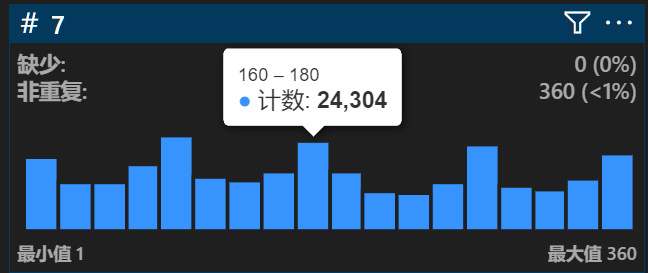
\includegraphics[width = 0.6\textwidth]{./img/7列统计信息.png}
    \caption{根据经纬度清理后第7列统计信息}
    \label{7-stat}
\end{figure}

除此之外,我们发现根据车号分组后有部分重复信息,因此去除重复的行,这部分清理了$14219$条数据。这可能是为了避免GPS信号未正常接收采取的数据冗余策略,但清理掉的数据占比较小,这一猜测或许并不靠谱。

进一步观察第5列的数据分布,最大值为123,除去数值为$0$的数据后数据分布如图\ref{4-stat},速度在80以下的占比较高,超过80的数据量较小,但在$[100,120]$范围内仍有相当数量的数据。因此我们猜测此列是速度信息,在非高速路段速度在$80$以下,高速路段速度在$[100,120]$(和现实中货车高速限速$100$或$110$以及存在小幅度超速现象是相符合的)。进一步我们取出某个车号,观察该辆车所有的数据信息(图\ref{v}),我们发现此列数据连续性较大,进一步印证了我们的猜测。这一信息可以通过将该列数据根据经纬度映射到地图后和高速路段、非高速路段上的分布进行验证。

\begin{figure}[!htb]
    \centering
    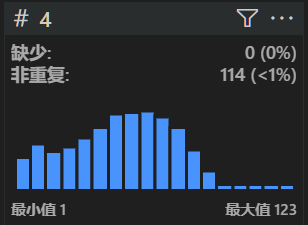
\includegraphics[width = 0.4\textwidth]{./img/4列统计信息.png}
    \caption{第4列统计信息}
    \label{4-stat}
\end{figure}

\begin{figure}[!htb]
    \centering
    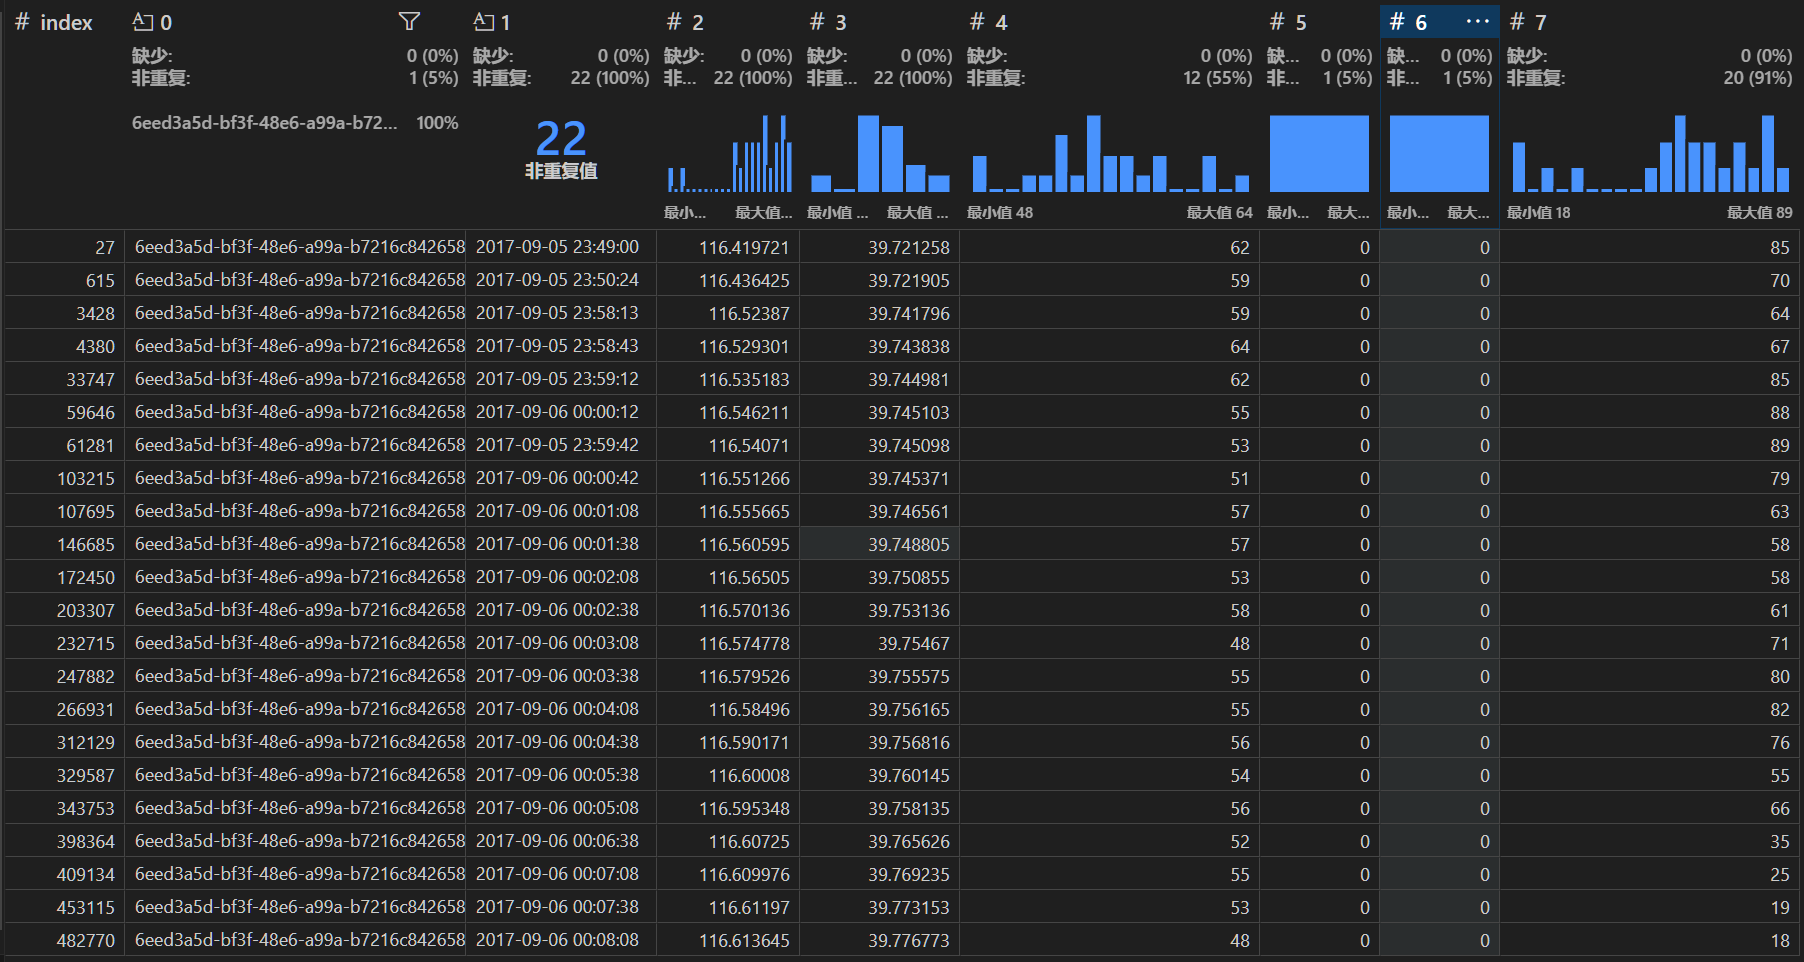
\includegraphics[width = 0.9\textwidth]{./img/速度推断信息.png}
    \caption{某辆车的数据总览和统计信息}
    \label{v}
\end{figure}

此时仍然剩余两列的列名未知,根据车号分组发现第5列数据在很多位置上和第4列相差很小,$33607$辆车中,只有$845$辆车的第6列数据存在两个或以上的值,其余$97.5\%$的车辆第6列的值是固定的,另一方面只有$1197$辆车的第6列数据中存在$1$,因此这一列的信息量并不大。至此,我们忽略这两列数据。

结合网络查找的资料\href{https://www.heywhale.com/mw/dataset/5f75ad252b83e00030b3f91d/file}{150万条营运车辆GPS数据}中对于每项数据的数据分布和统计信息,能够进一步印证关于速度和行驶方向这两列列名的猜测是正确的。

\subsection{数据清洗}

清除时间戳不在2017年9月5-6日的数据,清除数据$1367$条,剩余$33437$辆车的$362427$条数据。我们将上述流程分别应用于$100000$条数据和$1000000$条数据以及全量数据,每次清理和保留的数据的比例大致相当,因此我们可以认为这些数据清理流程是合理的。

表\ref{data}给出对于不同数据规模下每部分清理的数据和保留的数据的数量和所占的比例。
\begin{table}[h]
    \begin{center}
        \caption{数据清洗统计表}
        \label{data}
    \begin{minipage}{\textwidth}
    \centering
    \begin{tabular}{r|l|l|l|l}
        \hline \hline
    \textbf{数据量} & \textbf{100000} & \textbf{500000} & \textbf{1000000} & \textbf{67490000} \\ \hline
    车辆数 & 35017 & 43955 & 44923 & 74578 \\ \hline \hline
    经纬度清洗数量 & 27357 & 121987 & 239879 & 15911169 \\ \hline 
    剩余数据 & 72643 & 378013 & 760121 & 51578831 \\ \hline
    经纬度清洗比例\footnote{比例指当前阶段清洗数量占上一阶段剩余数据的比例,除最后一行的剩余数据比例指剩余数据占初始数据量的比例外,下同。} & 27.36\% & 24.40\% & 23.99\% & 23.58\% \\ \hline \hline
    重复数据清洗 & 2320 & 14219 & 28073 & 1879882 \\ \hline
    剩余数据 & 70323 & 363794 & 732048 & 49698949 \\ \hline
    重复数据清洗比例 & 3.19\% & 3.76\% & 3.69\% & 3.64\% \\ \hline \hline
    时间戳清洗 & 286 & 1367 & 2745 & 221973 \\ \hline
    剩余数据 & 70037 & 362427 & 729303 & 49476976 \\ \hline
    时间戳清洗比例 & 0.41\% & 0.38\% & 0.37\% & 0.45\% \\ \hline \hline
    停车数据清洗 & 48248 & 251557 & 507017 & 34059171 \\ \hline
    剩余数据 & 21789 & 110870 & 222286 & 15417805 \\ \hline
    停车数据清洗比例 & 68.89\% & 69.41\% & 69.52\% & 68.84\% \\ \hline \hline
    剩余车辆 & 6454 & 8377 & 9873 & 57693 \\ \hline
    剩余数据 & 21789 & 110870 & 222286 & 15417805 \\ \hline
    剩余数据比例 & 21.79\% & 22.17\% & 22.23\% & 22.84\% \\ 
    \hline \hline
    \end{tabular}
    \end{minipage}    

    \end{center}
    \end{table}

\section{聚集地和OD分析}

本节我们着手寻找货车前20名聚集地,并可视化呈现该聚集地的主要目的地和来源地。

\subsection{前20名聚集地}

首先需要注意的是,我们这里要求的聚集地,和第三次作业中的最密区域定义略有不同。聚集地偏向于车辆的聚集程度,对于同一辆车在某个区域内的多条数据,我们应该只计数一次。不过,这样就无法区分一辆车在一天之内多次到达某个区域的情况,因此我们需要对同一辆车的数据进行处理,如过两条数据的时间戳相差不超过$30$分钟,我们认为这是同一次行程,只计数一次;如果相差超过$30$分钟,我们认为这是两次行程,计数两次。

在具体的实现上,先对数据按照车号、时间戳两列排序,之后维护一个车号:时间戳的字典,每当有数据进入某一区域,如果车号不在字典中,或车号对应的时间戳超过$30$分钟,更新时间戳,计数加一;否则忽略这条数据。

根据附加要求,我们需要排除停车区,根据前面的分析,也就是清理掉所有速度$v\le 2 m /s$的数据。我们给出排除停车区前后的描点对比(图\ref{beijingGPS}),可以看到,停车数据对数据识别产生了相当大的影响。采用$500000$条数据时,剩余有效数据由$362427$条减少到$110870$条。

后续分析中,我们会明确指出是否排除了停车数据。

\begin{figure}[!htb]
    \centering
    \begin{subfigure}[b]{0.49\textwidth}
        \includegraphics[width=\textwidth]{./img/北京含停车.png}
        \caption{GPS数据地图描点(含静止车辆)}
        \label{beijing}
    \end{subfigure}
    \hfill
    \begin{subfigure}[b]{0.49\textwidth}
        \includegraphics[width=\textwidth]{./img/北京不含停车.png}
        \caption{GPS数据地图描点(不含静止车辆)}
        \label{beijingstop}
    \end{subfigure}
    \\
    \begin{subfigure}[b]{0.49\textwidth}
        \includegraphics[width=\textwidth]{./img/北京地图含停车.png}
        \caption{GPS数据地图描点(含静止车辆)}
        \label{beijingmap}
    \end{subfigure}
    \hfill
    \begin{subfigure}[b]{0.49\textwidth}
        \includegraphics[width=\textwidth]{./img/北京地图不含停车.png}
        \caption{GPS数据地图描点(不含静止车辆)}
        \label{beijingmapstop}
    \end{subfigure}
    \caption{GPS数据描点}
    \label{beijingGPS}
\end{figure}

我们还特意可视化了课堂上展示过的北野场桥的描点图图\ref{beiyechang}。这里采用了数据源的前$500$万条数据。

\begin{figure}[!htb]
    \centering
    \includegraphics[width = 0.9\textwidth]{./img/北野场桥.png}
    \caption{北野场桥}
    \label{beiyechang}
\end{figure}

\subsection{最密区域搜索}

\subsubsection{经度和纬度上间隔$1km$}

首先我们假定1平方公里范围的区域是约$1km\times 1km$的近似正方形,每条边分别与一条经线或纬线重合。根据北京市的经纬度范围,我们近似的认为上述近似正方形是纬度相差$\text{grid\_lat} = 0.0089927^\circ$,经度相差$\text{grid\_lon} = 0.011723^\circ$的四条经纬线围围成的。这两个数值是我们使用北京市中心的经纬度$39.906217°N, 116.3912757°E$分别向北和东走1km后变化的纬度和经度得到的。在北京市域小范围内,我们粗略的认为纬度变化引起的距离变化可以忽略不计。

至此,我们的目标已经转换为寻找前述的近似正方形。

\subsubsection{寻找最密区域,$n=500000$}


为了寻找数据最多的1平方公里区域,我们首先将北京市经度按照grid\_lat分为若干段,纬度按照gird\_lon分为若干段(也就是每隔1km),之后初始化一个数组,每个数组表示一个$2km\times 2km$的区域中数据点的个数。对于每个数据点,我们找到它所处的纬度和经度的区域,并为它所在的4个$2km\times 2km$区域\footnote{因为经纬度是按照$1km$分段的,所以相邻的$2km\times 2km$区域是有$1km$重叠的,那每个点被分到某两个经度和某两个纬度之间时,它其实处于4个$2km\times 2km$的区域。}的数据点个数都加一。这样,我们统计了这些$2km\times 2km$网格中数据点的个数。

接下来选择一个阈值$\alpha$,选择数据点区域占总数据量的比例大于$\alpha$的$2km\times 2km$区域,我们得到若干个参考区域。对于每个参考区域,我们以$100m$为步长,枚举所有的$121$个$1km\times 1km$区域,找出点数最多的区域$R$和点数$n$。

再计算$n$占总数据的比例$\beta$,搜索数据点区域占总数据量的比例大于$\beta$的$2km\times 2km$区域,我们得到若干个备选区域。对于每个备选区域,重复以$100m$为步长,枚举所有的$121$个$1km\times 1km$区域,找出点数最多的区域$R_1$和点数$n_1$,我们发现$n_1\le n$,从而前面的区域$R$就是我们要找的数据最密区域。

我们可以证明这样的结果在步长为$100m$时是正确的:因为我们第二次根据阈值$\beta$搜索时,找到了所有点数超过$R$的$2km\times 2km$区域(备选区域),而我们这里的$R$仅是$1km\times 1km$的区域,所以其他没有被列入备选区域的子区域不可能出现点数$\ge n$的$1km\times 1km$区域。对于每个备选区域,我们直接枚举这些区域中数据最多的$1km\times 1km$区域,他们都比$R$少,那么$R$的数据点就是最多的。

在总数据量为$500000$时,我们使用参数$\alpha=0.005$,第一次找到的参考区域有一个,点数$n = 3650$,得到$\beta$,再得到三个备选区域(图\ref{denseResult}),枚举后发现前面找到的$R$就是数据最密区域(图\ref{denseLarge})。$$ R = (39.80600289, 39.81499559) \times (116.3326001, 116.3443231) $$

\subsubsection{全量数据最密区域}

本部分的代码见allTruckGps.ipynb中“大区域”一节。

我们使用全量数据,类似流程可以得到相同结果(图\ref{denseResultAll},\ref{denseLargeAll}),具体的操作可见allTruckGps.ipynb,其中参数$\alpha=0.047, n = 452968$,$R$同上。至此,我们找到了全量数据的最密集1平方公里区域。而且非常明显的,使用全量数据后,路网连线被非常清晰的可视化(./html/denseRegion.html)。

\begin{figure}[!htb]
    \centering
    \begin{subfigure}[b]{0.7\textwidth}
        \includegraphics[width=\textwidth]{./img/最密区域.png}
        \caption{数据量$500000$,含停车}
        \label{denseResult}
    \end{subfigure}
    \\
    \begin{subfigure}[b]{0.7\textwidth}
        \includegraphics[width=\textwidth]{./img/最密区域all.png}
        \caption{全量数据,含停车}
        \label{denseResultAll}
    \end{subfigure}
    \caption{最密区域结果}
    \label{denseR}
\end{figure}

\begin{figure}[!htb]
    \centering
    \begin{subfigure}[b]{0.49\textwidth}
        \includegraphics[width=\textwidth]{./img/最密大含停车.png}
        \caption{数据量$500000$,含停车}
        \label{denseLarge}
    \end{subfigure}
    \hfill
    \begin{subfigure}[b]{0.49\textwidth}
        \includegraphics[width=\textwidth]{./img/最密大all含停车.png}
        \caption{全量数据,含停车}
        \label{denseLargeAll}
    \end{subfigure}
    \caption{最密区域($1km\times 1km$)可视化和路网连线}
    \label{denseL}
\end{figure}

\subsection{密集区与非密集区划分}

得益于我们划分网格的方法,这部分相对来说非常简单,我们只需要根据每个格点的数据绘制热力图即可。需要注意的是,大多数数据值取值较小,我们需要手动指定热力图的vmax参数,否则热力图将是漆黑一片。即使我们将vmax参数设置为$5$,热力图中亮色仍然较少(图\ref{hotSmall})。

为了获得更好的表示,我们尝试在之前间隔\footnote{注意这里的间隔只是相邻两个网格边界的距离,网格的边长仍然是$2km$,相邻网格之间仍然存在重叠。}$1km$的网格上绘制热力图,这次我们将vmax设置到$30000$时,就能得到非常好的结果(图\ref{hot})。

\begin{figure}[!htb]
    \centering
    \begin{subfigure}[b]{0.49\textwidth}
        \includegraphics[width=\textwidth]{./img/热力图小区域.png}
        \caption{小区域网格热力图}
        \label{hotSmall}
    \end{subfigure}
    \hfill
    \begin{subfigure}[b]{0.49\textwidth}
        \includegraphics[width=\textwidth]{./img/热力图.png}
        \caption{大区域网格热力图}
        \label{hot}
    \end{subfigure}
    \caption{热力图,用以区分数据密集区与非密集区}
    \label{hotL}
\end{figure}

如果想要更加准确的分界线,取合适的阈值(比如vmax/3)将网格数据点二值化为$0$和$1$,$0,1$变化的位置就是分界线。

\section{总结与反思}

有了上次作业的教训,这次作业起步较早,每天完成一小部分,经过接近两周的鏖战,基本完成了所有要求的内容。刚把数据拿到手时确实存在束手无策之感,但在一点一点解决当下问题的过程中,都能够想到很好的方法实现作业要求,还利用完成作业中搜集到的其他知识给出了一些其他的结果。

邓老师课上对数据处理整个流程的讲解,也让我更加明确了完成作业的步骤。

在数据分析过程中,时刻注意更精妙的算法、时间复杂度的分析等,能够帮助我们将方法推广到更广阔的范围中。

不过纵观整个流程来讲,代码文件还是没能得到很好的组织,最后运行全量数据时仍然需要新开一个文件,排除不必要运算以节省时间。

对于数据处理目标1,如果能将程序封装为命令行查询程序,显然是更加直观的结果,不过受限于时间,本次作业中并没有实现。

总的来说,这次作业增加了我对大规模数据处理的经验和信心。

\end{document}

